
%%% Local Variables: 
%%% mode: latex
%%% TeX-master: t
%%% End: 

\chapter{基于 $k$-CBP 碰撞检测算法}
\label{cha:kcbp-collision-detection}

碰撞检测算法是计算机图形学、计算机动画等领域里必不可少的。
本章提出了基于~$k$-CBP~的碰撞检测算法,算法首先对输入的网格模型进行预处理,构造模型的~AABB~包围体、$k$-CBP,
当进行碰撞检测时,首先判断~AABB~是否相交,若相交再进行~$k$-CBP~之间的相交测试,再次相交再进行实际模型的相交测试。再进行实际模型的相交测试时,利用了~AABB~树形结构进行判断剪枝。
在凸包围~$k$~面体之间分别用~AABB~树的方式和基于~GJK~算法两种方式进行,实验结果表明本文提出的方法能够有效加速碰撞检测算法。

本章后续部分的内容组织如下:
第一小节介绍~$k$-CBP~之间的相交测试算法,
第二小节介绍三角网格的相交测试算法,
第三节介绍总体的算法流程,
最后一节为实验结果的分析。


\section{$k$-CBP 的相交测试算法}
\label{sec:kcbp:cd}

在所有基于包围体的碰撞检测算法中,都是利用了包围体的相交测试比直接用原始模型相交测试更简单以提升算法的整体效率,包围体的相交测试是非常重要的一个步骤。
与其他基于包围体的碰撞检测算法一样,本文基于~$k$-CBP~的算法也是先进行~$k$-CBP~的相交测试,若~$k$-CBP~相交,再进行原始模型的相交测试。
$k$-CBP~之间的相交测试以两种方法实现,一种是将构造的~$k$-CBP~进行空间划分,构造~$k$-CBP~的~AABB~树,再基于~AABB~树进行相交测试,详细划分原则等算法见第~\ref{subsec:kcbp:cd:aabb}~;
另一种是基于凸多面体的相交测试算法~GJK~,详细算法见第~\ref{subsec:kcbp:cd:gjk}节。

\subsection{基于 AABB 树的算法}
\label{subsec:kcbp:cd:aabb}

AABB~包围体是碰撞检测算法过程中一种常用的包围体,构造模型的~AABB~包围体树能够有效提高模型的求交或碰撞检测过程。
本文将构造得到的~$k$-CBP~视为普通的三角网格模型,采取一种自上而下的构造~AABB~包围体树的方法,顶层包围体为所有三角网格的包围体的并集,然后按照包围体跨度最大的维度进行划分成两个子节点,然后再对每个子节点进行递归划分。
具体算法如算法~\ref{alg:aabbtree:build}~所示。

\begin{algorithm}[htbp]
\small
\caption{AABB~树的构造}
\label{alg:aabbtree:build}
\begin{algorithmic}[1]
\Require
原始三角网格 $primitives$ 和下标 $first, last$
\Ensure
AABB~树的根节点 $root$

\Function{ConstructAABBTree}{$primitives, first, last$}
  \State $root \gets \Call{constructNode()}{}$ 
  \State $root.primitives \gets primitives$
  %\State $root.box \gets \emptyset $
  \For{$i = first \to last$}
      \State $root.box \gets root.box \cup primitives[i].box$
      \Comment{求每个三角网格的~AABB~的并集}
  \EndFor

  \State $size \gets primitives.size$  
  \If {$size = 1$}
  \State \Return $root$
  \EndIf

  \State $axis \gets \Call{longestAixs}{root.box}$
  \Comment {计算包围体跨度最大的轴}
  \State {$\Call{sort}{primitives, axis}$}
  \Comment {按照 $axis$ 对 $primitives$ 排序}
  
  \If {$size = 2 $}
      \State  {$root.left \gets \Call{constructNode()}{}$}
      \State  {$root.left.primitives \gets primitives[0]$}
      \State  {$root.left.box \gets primitives[0].box$}
      \State  {$root.right \gets \Call{constructNode()}{}$}
      \State  {$root.right.primitives \gets primitives[1]$}
      \State  {$root.right.box \gets primitives[1].box$}
      \State \Return $root$
  \EndIf
  \State $half \gets size / 2 $
  \State $root.left \gets \Call{ConstructAABBTree}{primitives, first, half}$
  \State \Comment{前一半作为其中一个叶子节点,继续递归构造}
  \State $root.right \gets \Call{ConstructAABBTree}{primitives, half+1, size}$ \Comment{后一半继续递归构造}
  \State \Return $root$
\EndFunction
\end{algorithmic}
\end{algorithm}

为了使生成的~AABB~包围体树更加平衡,因此划分策略为两个子节点包含相同数量的三角网格。划分轴采用沿着坐标轴方向节点跨度最大的轴进行划分,在对三角网格进行排序时,通常可选择三角网格中心位置的某轴向坐标值进行排序,
因为本文的策略为平衡二叉树策略,两个孩子节点包含三角网格数量一致,因此该点的选择不会对总体划分产生较大影响,只会影响划分轴边缘的三角网格,因此本文仅仅简单选择三角网格第一个坐标点的轴向坐标轴进行排序。

假设算法~\ref{alg:aabbtree:build}~的时间复杂度为~$T(n)$~,则有
\begin{equation}
  T(n) = O(n \log n ) + 2T(\frac{n}{2}),
\label{equa:aabbtree:build}
\end{equation}
公式~\ref{equa:aabbtree:build}~中~$O(n \log n)$~为算法中根据某坐标轴排序的耗费,根据主定理得此构造包围体树的整体算法时间复杂度~$T(n)=O(n\log^2n)$~,文献~\onlinecite{ericson2005real}~中提到可以用一种~$O(n)$~的算法替代其中的排序操作,使得整体复杂度为~$O(n\log n)$。

生成两个~$k$-CBP~的~AABB~包围体树后,当进行碰撞检测时,将采用算法~\ref{alg:aabbtree:traverse:iterator}~的迭代算法进行遍历判断。
从顶层~AABB~节点开始,若两个节点的~AABB~包围体相交,则进行深度优先遍历其孩子节点,当到达叶子节点时,再进行原生几何(本文中的~$k$-CBP~多边形网格,为了统一转化成与输入模型一致的三角网格)进行相交测试的判断,$k$-CBP~相交后,进行真实模型的相交测试也通过此方法进行。

\begin{algorithm}[htbp]
\small
\caption{基于AABB~树碰撞检测迭代算法}
\label{alg:aabbtree:traverse:iterator}
\begin{algorithmic}[1]
\Require
两棵~AABB~树的根节点 $rootA, rootB$
\Ensure
是否相交

\Function{TraverseDetection}{$rootA, rootB$}
  \State $p \gets \Call{initStack()}{}, q \gets \Call{initStack()}{}$  \Comment{初始化两个栈,用于记录待判断的~AABB~节点对}
  \State $p.\Call{Push}{rootA}, q.\Call{Push}{rootB}$  
  
  \While {$! p.\Call{empty()}{} ~~\textbf{and}~~ !q.\Call{empty()}{}$}
      \State $nodeA \gets p.\Call{Pop()}{}$
      \State $nodeB \gets q.\Call{Pop()}{}$
      \State $c \gets \Call{Intersect}{nodeA.box, nodeB.box}$ \Comment {判断两个节点的~AABB~包围体是否相交}
      \If {$c = \textbf{False}$}
          \State \textbf{Continue} \Comment{节点~AABB~不相交,则过滤到这两个节点及其孩子节点}
      \EndIf
      \If {$nodeA.\Call{isLeaf()}{}$}
          \If {$nodeB.\Call{isLeaf()}{}$}
              \Comment{两个叶子节点的原始几何进行相交测试} 
              \ForAll {$p_1 \in nodeA.primitives$}
                  \ForAll {$p_2 \in nodeB.primitives$}
                      \If {$\Call{Intersect}{p_1, p_2} = \textbf{True} $}
                          \State \Comment {按照第~\ref{sec:intersection:triangles}~节中的算法进行原始三角网格相交测试}
                          \State \Return \textbf{True} \Comment{若相交就直接返回True}
                      \EndIf
                  \EndFor
              \EndFor
          \Else  \Comment{nodeB~节点有孩子节点}
              \State $p.\Call{push}{nodeA}, q.\Call{push}{nodeB.left}$
              \State $p.\Call{push}{nodeA}, q.\Call{push}{nodeB.right}$
          \EndIf
      \Else \Comment{nodeA~节点有孩子节点}
          \If {$nodeB.\Call{isLeaf()}{}$}
              \Comment{nodeB~是叶子节点}
              \State $p.\Call{push}{nodeA.left}, q.\Call{push}{nodeB}$
              \State $p.\Call{push}{nodeA.right}, q.\Call{push}{nodeB}$
          \Else
              \Comment{nodeA~和~nodeB~都有叶子节点} 
              \State $p.\Call{push}{nodeA.left}, q.\Call{push}{nodeB.left}$
              \State $p.\Call{push}{nodeA.left}, q.\Call{push}{nodeB.right}$
              \State $p.\Call{push}{nodeA.right}, q.\Call{push}{nodeB.left}$
              \State $p.\Call{push}{nodeA.right}, q.\Call{push}{nodeB.right}$
          \EndIf
      \EndIf
  \EndWhile
  \State \Return \textbf{False} \Comment{遍历完毕也没有检测到原始三角网格相交,则返回False}
\EndFunction
\end{algorithmic}
\end{algorithm}

算法~\ref{alg:aabbtree:traverse:iterator}~中,底层叶子节点包含的原始三角网格数量与树的高度相关,对于相同的模型,树的高度越低,叶子节点包含三角网格数量也就越多,
且叶子节点测试的时间复杂度为~$O(m^2)$,$m$~为叶子节点包含的三角网格数量,一般而言在存储允许的情况下都尽量使得最底层叶子节点仅包含1个或少数几个三角形,以减少底层叶子节点三角网格两两测试的时间复杂度。

当在运动场景中的模型进行碰撞检测时,需要对~$k$-CBP及模型的~AABB~包围体树进行更新,本文采用一种近似的算法进行计算,详细将在第~\ref{sec:cd:baseon:kcbp}~节中介绍。

\subsection{基于 GJK 的算法}
\label{subsec:kcbp:cd:gjk}

GJK~算法是~E.G.Gilbert,D. W. Jonhson~和S.S. Keerthi(取三位作者姓名首字母作为算法名称的缩写)~等人在1988年发表的一种用于计算三维欧式空间中两个凸集合点之间的距离\cite{gilbert1988fast},后常用于凸体之间的碰撞检测算法\cite{bergen1999fast}。本文也利用此算法用于计算两个凸包围多面体~$k$-CBP~之间的相交测试。

GJK~算法需要用到闵科夫斯基和(Minkowski Sum)如下定义:两个点集~A~和~B~,其~Minkowski~和为
\begin{equation}
  A + B = \{ a + b | a \in A, b \in B\},  
  \label{}
\end{equation}
将相应的加号改为减号得到~Minkowski~差,即~$A - B = \{ a - b | a \in A, b \in B\}$,GJK~算法的核心基础在于若两个凸体相交,则其~Minkowski~差必包含原点,因为若~A~和~B~相交即~A~和~B~必含有公共交集,
即至少含有一点同时属于~A~和~B~,该点的~Minkowski~差即为原点~$(0, 0)$,
更加详细的证明过程可参考文献~\onlinecite{gilbert1988fast,bergen1999fast}。下面将以一个二维例子阐述此思想。

\begin{figure}[htbp]
\centering
\subcaptionbox{相交\label{fig:gjk:example:intersection}}{
  \includegraphics[width=.48\textwidth]{gjkIntersection.tikz}
} 
\subcaptionbox{不相交\label{fig:gjk:example:nonIntersection}}{
  \includegraphics[width=.48\textwidth]{gjkNonIntersection.tikz}
}
\caption{二维~GJK~算法示例}
\label{fig:gjk:example:2d}
\end{figure}

如图~\ref{fig:gjk:example:2d}~所示,图~\ref{fig:gjk:example:intersection}~中,四边形~$DEFG$~四个点坐标分别为$D(-4, 2), E(-2.5, 2), F(-2.5, 3.5), G(-4, 3.5)$,
三角形~$ABC$~的坐标分别为~$A(-3, 1), B(-1,3), C(-3, 3)$~,其~Minkowski~差如式~\ref{equa:gjk:example:mink:diff}~所示,

\begin{equation}
\label{equa:gjk:example:mink:diff}
\Box_{DEFG} - \bigtriangleup_{ABC} = \left\{ 
  \begin{array}{l}
    (0.5, 1),  (-1.5, 0.5),  (0.5, 2.5), (-1, 2.5), (-3, -1), (-1, -1), \\
    (0.5, 0.5), (-1, 1), (-3, 0.5), (0.5, -1), (-1.5, -1), (-1, 0.5)
  \end{array}
    \right\}  
\end{equation}
四边形~$DEFG$~与三角形~$ABC$~相交,该~Minkowski~差构成的多边形~$H_1H_2H_3H_4H_5$包含原点~$\bm{O}$。而图~\ref{fig:gjk:example:nonIntersection}~中,
四边形~$DEFG$~坐标不变,三角形坐标变为~$A(-3, 1), B(-1, 1), C(-1,3)$,其~Minkowski~差如式~\ref{equa:gjk:example:mink:diff2}~所示,

\begin{equation}
\label{equa:gjk:example:mink:diff2}
\Box_{DEFG} - \bigtriangleup_{A'B'C'} = \left\{ 
  \begin{array}{l}
   (0.5, 1), (-1.5, 1),(0.5, 2.5)  , (-1.5, -1), (-1, 2.5),(-3, 2.5), \\ 
   (-1.5, 2.5), (-3, 1), (-1.5, 0.5), (-3, 0.5), (-1, 1),(-3, -1) 
  \end{array}
  \right\}  
\end{equation}
四边形~$DEFG$~与三角形~$A'B'C'$~不相交,该~Minkowski~差构成的多边形~$H_1'H_2'H_3'H_4'H_5'$不包含原点~$\bm{O}$。

通过该方法可将两个凸多边形或多面体是否相交转化为其~Minkowski~差是否包含原点,假设两个凸多边形或多面体分别有~$m$~和~$n$~个点,则直接计算其~Minkowski~差的时间复杂度为~$O(m \cdot n)$。
GJK~算法并不直接计算其~Minkowski~差,而是采取一种迭代的算法计算其~Minkowski~差一步一步向逼近原点,在有限步内若包含原点则原凸多边形或凸多面体相交反之不相交,而该迭代算法能在有限步内完成。

GJK~算法中定义支持映射(Support Mapping)函数为将给定的方向~$\bm{d}$~映射为凸多边形或多面体中沿着~$\bm{d}$~方向最远的点,该点称为支持点(Support Point),用符号~$Support(\bm{d})$~表示,
该概念与本文第~\ref{sec:search:planes}节中搜索截面中的最大投影值点一致。设~$\mathbb{A}$~和~$\mathbb{B}$~的~Minkowski~差为~$\mathbb{D} = \mathbb{A}-\mathbb{B}$~,
则~$Support_\mathbb{D}(\bm{d}) = Support_\mathbb{A}(\bm{d}) - Support_\mathbb{B}(-\bm{d})$,这样能使得
~D~围成的区域更大并尽可能的包含原点。

GJK~算法采用如下的流程进行迭代计算两个凸多面体~$\mathbb{A}$~和~$\mathbb{B}$~是否相交:
%\cite{ericson2005real}

\begin{enumerate}[(1)]
  \item 任选方向~$\bm{d}$~计算~$Support_\mathbb{D}(\bm{d}) = Support_\mathbb{A}(\bm{d}) - Support_\mathbb{B}(-\bm{d})$,即任意从~$\mathbb{A}$~和~$\mathbb{B}$~的~Minkowski~差中选择一点,加入集合~$\bm{S}$;
  \item 计算~$ConvxHull(S)$~中,具有最小二范数的点(离原点最近的点)~$D$; 
  \item 如果~$D$~是原点本身或~$ConvxHull(S)$包含原点,则表明$\mathbb{A}$~和~$\mathbb{B}$~相交,停止迭代;
  \item 规约集合~$\bm{S}$~,使得~$\bm{S}$~中是满足~$D$~属于其凸包的最小的集合;
  \item 更新方向~$\bm{d} = -\bm{D}$~,并计算~$Support_\mathbb{D}(\bm{d}) = Support_\mathbb{A}(\bm{d}) - Support_\mathbb{B}(-\bm{d})$;
  \item 如果有新的$Support_\mathbb{D}(\bm{d})$~产生,则添加至集合~$\bm{S}$~并从第(2)步继续迭代,否则结束迭代,且$\mathbb{A}$~和~$\mathbb{B}$~不相交。
\end{enumerate}

具体而言,仍以图~\ref{fig:gjk:example:intersection}~为例,令四边形~$DEFG$~为~$\mathbb{A}$~,三角形~$ABC$~为~$\mathbb{B}$~,

第一次迭代令~$\bm{d_1} = (1,0)$,如图~\ref{fig:gjk:example:intersection:step1}~所示,
\begin{equation}
  \begin{array}{ll}
    Support_\mathbb{D}(d_1) & = Support_\mathbb{A}(\bm{d_1}) - Support_\mathbb{B}(-\bm{d_1}) \\
                            & = E(-2.5, 2) - A(-3,1) \\
                            & = D_1(0.5, 1)
  \end{array}
  \label{euqa:gjk:step1}
\end{equation}

\begin{figure}[htbp]
\centering
\subcaptionbox{第一次迭代\label{fig:gjk:example:intersection:step1}}{
  \includegraphics[width=.48\textwidth]{gjkExampleIntersectionStep1.tikz}
} 
\subcaptionbox{第二次迭代\label{fig:gjk:example:intersection:step2}}{
  \includegraphics[width=.48\textwidth]{gjkExampleIntersectionStep2.tikz}
}
\subcaptionbox{第三次迭代\label{fig:gjk:example:intersection:step3}}{
  \includegraphics[width=.48\textwidth]{gjkExampleIntersectionStep3.tikz}
}
\caption{二维~GJK~算法迭代示例(相交情况)}
\label{fig:gjk:example:2d:intersection:iterator}
\end{figure}

此时,$\bm{S} = \{D_1(0.5, 1)\}$,第二次迭代取~$\bm{d_2}=-\bm{D_1}=(-0.5, -1)$,
\begin{equation}
  \begin{array}{ll}
  Support_\mathbb{D}(d_2)  & = Support_\mathbb{A}(\bm{d_2}) - Support_\mathbb{B}(-\bm{d_2}) \\
    & = D(-4, 2) - B(-1, 3) \\
    & = D_2(-3, -1)
  \end{array}
  \label{euqa:gjk:step2}
\end{equation}

此时,$\bm{S} = \{D_1(-0.5, 1), D_2(-3, -1)\}$,第三次迭代,计算~$ConvexHull(S)$~中最小二范数的点为~$I(-4/13, 7/13)$~,
并令~$\bm{d_3}=-\bm{I}=(4/13, -7/13)$,
\begin{equation}
  \begin{array}{ll}
  Support_\mathbb{D}(d_3)  & = Support_\mathbb{A}(\bm{d_3}) - Support_\mathbb{B}(-\bm{d_3}) \\
    & = E(-2.5, 2) - C(-3, 3) \\
    & = D_3(0.5, -1)
  \end{array}
  \label{euqa:gjk:step3}
\end{equation}

此时$\bm{S} = \{D_1(0.5, 1), D_2(-3, -1), D_3(0.5, -1)\}$,如图~\ref{fig:gjk:example:intersection:step3}~所示,$ConvexHull(S)$~为阴影部分包含原点,结束迭代,$\mathbb{A}$~和~$\mathbb{B}$~相交。

再以图~\ref{fig:gjk:example:nonIntersection}~为例,设三角形$\mathbb{B'} = A'B'C'$,该例前两次迭代与上例相同,此处省略直接从第三次迭代起,

\begin{figure}[htbp]
\centering
\subcaptionbox{第三次迭代\label{fig:gjk:example:nonIntersection:step3}}{
  \includegraphics[width=.48\textwidth]{gjkExampleNonIntersectionStep3.tikz}
} 
\subcaptionbox{第四次迭代\label{fig:gjk:example:nonIntersection:step4}}{
  \includegraphics[width=.48\textwidth]{gjkExampleNonIntersectionStep4.tikz}
}
\caption{二维~GJK~算法迭代示例(不相交情况)}
\label{fig:gjk:example:2d:intersection:iterator}
\end{figure}

第三次迭代,$\bm{S} = \{(D_1', D_2') \}$,此时~$\bm{d_3}=-\bm{I}=(4/13, -7/13)$,
\begin{equation}
  \begin{array}{ll}
  Support_\mathbb{D}(d_3)  & = Support_\mathbb{A}(\bm{d_3}) - Support_\mathbb{B'}(-\bm{d_3}) \\
    & = E(-2.5, 2) - C'(-1, 3) \\
    & = D_3'(-1.5, -1)
  \end{array}
  \label{euqa:gjk:non:step3}
\end{equation}

此时$\bm{S} = \{D_1'(0.5, 1), D_2'(-3, -1), D_3(-1.5, -1)\}$,如图~\ref{fig:gjk:example:nonIntersection:step3}~所示,$ConvexHull(S)$~并不包含原点,继续迭代,

计算~$\bm{S}$~中二范数最小的点为~$I_2(-1/4, 1/4)$~,并规约集合~$\bm{S}$,点~$D_2'$~可去掉,
变为$\bm{S} = \{ (D_1'(0.5, 1), D_3'(-1.5, -1)\}$,并另$\bm{d}_4 = -I_2 = (1/4, -1/4)$,
\begin{equation}
  \begin{array}{ll}
  Support_\mathbb{D}(d_4)  & = Support_\mathbb{A}(\bm{d_4}) - Support_\mathbb{B'}(-\bm{d_4}) \\
    & = E(-2.5, 2) - C'(-1, 3) \textbf{~or~} A'(-3, 1)  \\
    & = D_3'(-1.5, -1) \textbf{~or~} D_1'(0.5, 1)
  \end{array}
  \label{euqa:gjk:non:step4}
\end{equation}

此时,没有新的~$Support_\mathbb{D}(\bm{d})$~产生,结束迭代,$\mathbb{A}$~和~$\mathbb{B}$~不相交。

在实际计算过程中,并不需要计算离原点最近(二范数最小)的点的坐标,只需选择垂直已有方向再进行判断选择方向即可,以图~\ref{fig:gjk:example:intersection:step3}~为例,
此时~$\overrightarrow{D_1D_2} = D_2(-3, -1) - D_1(0.5, 1) = (-3.5, -2)$,此时只需令~
$\bm{d_3'} = D_1D_2 \times D_1O \times D_1D_2 = -(D_1D_2 \cdot D_1O)D_1D_2 +
(D_1D_2 \cdot D_1D_2)D_1O = (5,-8.75)$($\bm{a} \times \bm{b} \times \bm{c} =
-(\bm{c}\cdot\bm{b})\bm{a}+(\bm{c}\cdot\bm{a})\bm{b})$),
\begin{equation}
  \begin{array}{ll}
  Support_\mathbb{D}(d_3')  & = Support_\mathbb{A}(\bm{d_3'}) - Support_\mathbb{B'}(-\bm{d_3'}) \\
    & = E(-2.5, 2) - C(-3, 3) \\
    & = D_3(0.5, -1) 
  \end{array}
\end{equation}
得到的~$Support_\mathbb{D}(d_3')$~仍为~$D_3(0.5,-1)$,与选择二范数最小点~$I$~所代表的方向达到相同的结果,因为选择二范数最小点的坐标代表方向与该垂直方向相同,因此结果一致。

\begin{enumerate}[(1)]
  \item 通过$\bm{d}_3'$~得到的支持点$\bm{D}_3$中,$\bm{d}_3' \cdot OD_3 = (5, -8.75) \cdot (0.5, -1) = 11.25 > 0$~表明通过~$\bm{d}_3'$~方向到支持点的方向覆盖了原点,
即原点在线段~$D_1D_2$~线段的右下方;
  \item $\overrightarrow{D_3D_1}$~垂直并指向阴影部分面积方向为~$\overrightarrow{P_{D3D1}}=\overrightarrow{D_3D_1} \times \overrightarrow{D_3D_2} \times \overrightarrow{D_3D_1} = (-14, 0)$,此时,$\overrightarrow{P_{D3D1}} \cdot D_3O = (-14, 0) \cdot (-0.5, 1) = 7 < 0$~表明原点~$\bm{O}$~在~$\overrightarrow{P_{D3D1}}$的正方向即线段~$D3D1$~的左边;
  \item 同时,$\overrightarrow{D_3D_2}$~垂直并指向阴影部分面积方向为~$\overrightarrow{P_{D3D2}}=\overrightarrow{D_3D_2}
\times \overrightarrow{D_3D_1} \times \overrightarrow{D_3D_2} = (0, 24.5)$
且~$\overrightarrow{P_{D3D1}} \cdot D_3O = (0, 24.5) \cdot (-0.5, 1) = 24.5 > 0$~表明原点~$\bm{O}$~在~$\overrightarrow{P_{D3D2}}$的正方向即线段~$D3D2$~的上边;
\end{enumerate}
以上三个条件全部满足,即原点~$\bm{O}$~被阴影部分所覆盖,即~$\mathbb{A}$~和~$\mathbb{B}$~的~Minkowski~差包含原点即可确定~$\mathbb{A}$~和~$\mathbb{B}$~相交,结束迭代。

相应的以图~\ref{fig:gjk:example:nonIntersection:step3}~为例,其结果仍一样。
\begin{equation}
  \begin{array}{ll}
  Support_\mathbb{D}(d_3')  & = Support_\mathbb{A}(\bm{d_3'}) - Support_\mathbb{B'}(-\bm{d_3'}) \\
    & = E(-2.5, 2) - C'(-1, 3) \\
    & = D_3'(-1.5, -1) 
  \end{array}
\end{equation}
图~\ref{fig:gjk:example:nonIntersection:step3}~中,
上一步通过~$\bm{d}_3'$~得到的支持点为~$D_3'(-1.5, -1)$,且$\overrightarrow{D_3'D_1'}$~垂直并指向阴影部分面积方向为~$\overrightarrow{P_{D_3'D_1'}}
\times \overrightarrow{D_3'D_2'} \times \overrightarrow{D_3'D_1'} =
(-2,-2)*(-3) + 8*(-1.5, 0) = (-6, 6)$,此时
~$\overrightarrow{P_{D3'D1'}} \cdot D_3'O = (-6, 6) \cdot (1.5, 1) = -3 < 0$~表明下一次迭代方向需要以~$\overrightarrow{P_{D3'D1'}}$~的反方向开始,此时点~$D_2'$~可以规约掉,
即~$\bm{d}_4'= (6, -6)$,以此方向得到的支持点~$D_1'(0.5, 1)$,
此时,$\bm{d}_4' \cdot OD_1 = (6, -6) \cdot (0.5, 1) = -3 < 0 $ 表明通过~$\bm{d}_4'$~方向到支持点覆盖的区域没有包含原点,即可排除相交。

具体的算法如算法~\ref{alg:gjk}~所示,文献~\onlinecite{bergen1999fast}~证明了集合~$\bm{S}$~中在三维空间最多只包含4个点,且算法最终会收敛。
在实际实现过程中可以根据需求设定最大迭代次数,达到后或者认为没找到相交点或者采取保守态度进行下一步验证。

\begin{algorithm}[htbp]
\small
\caption{基于~GJK~的~$k$~CBP~相交检测算法}
\label{alg:gjk}
\begin{algorithmic}[1]
\Require
$k$-CBP~ $k\texttt{-}CBP_1, k\texttt{-}CBP_2$
\Ensure
是否相交
\Function{KCBPDetectionBasedOnGJK}{$k\texttt{-}CBP_1, k\texttt{-}CBP_2$}
    \State $\bm{d} \gets \Call{initNormal}$
    \State $\bm{D} \gets \Call{Support}{k\texttt{-}CBP_1, k\texttt{-}CBP_2, \bm{d}}$
    \State $S \gets \{p\}$
    \State $iter \gets 1 , \bm{d} \gets -\bm{d}$
    \While{$inter++ < MaxIter$}
        \State $\bm{D} \gets \Call{Support}{k\texttt{-}CBP_1, k\texttt{-}CBP_2, \bm{d}}$
        \If {$\bm{D} \cdot \bm{d} < 0 $}
            \State \Return \textbf{False}
        \EndIf
        \State $S \gets S \cup \bm{D}$
        \State $ contains \gets \Call{CheckContainUpdate}{S, \bm{d}}$ \Comment{检测是否包含原点,对集合~$S$~进行规约,并获取下一次迭代的方向~$\bm{d}$}
        \If {$contains$}
            \State \Return \textbf{True} \Comment{包含原点,直接返回相交,否则继续迭代}
        \EndIf
    \EndWhile
    \State \Return \textbf{False} \Comment{达到最大迭代次数,根据需求返回相交或者不相交}
\EndFunction
\end{algorithmic}
\end{algorithm}

算法~\ref{alg:gjk}~第~12~行~$CheckContainUpdate$~子过称需检测~$\bm{S}$~是否包含原点,必要时进行规约并获取下一次迭代方向,以上两个例子已经对二维情况进行分析,
具体三维实现可以参考文献~\onlinecite{bergen1999fast}。


\section{三角网格的相交测试算法}
\label{sec:intersection:triangles}

所有针对三角网格模型的碰撞检测算法最终都离不开三角网格的相交测试,不管模型是用何种包围体采用几何或者代数的方法都需要进行三角网格的相交测试。本文将利用一种几何代数相结合的方法进行三角网格之间的相交测试。
具体而言,假设两个不同面的三角形所在平面交于直线~$\bm{L}$~,两个三角形位置关系分为相交或者不相交两种情况,如图~\ref{fig:two:triangle:ui}所示。

\begin{figure}[htbp]
  \centering
    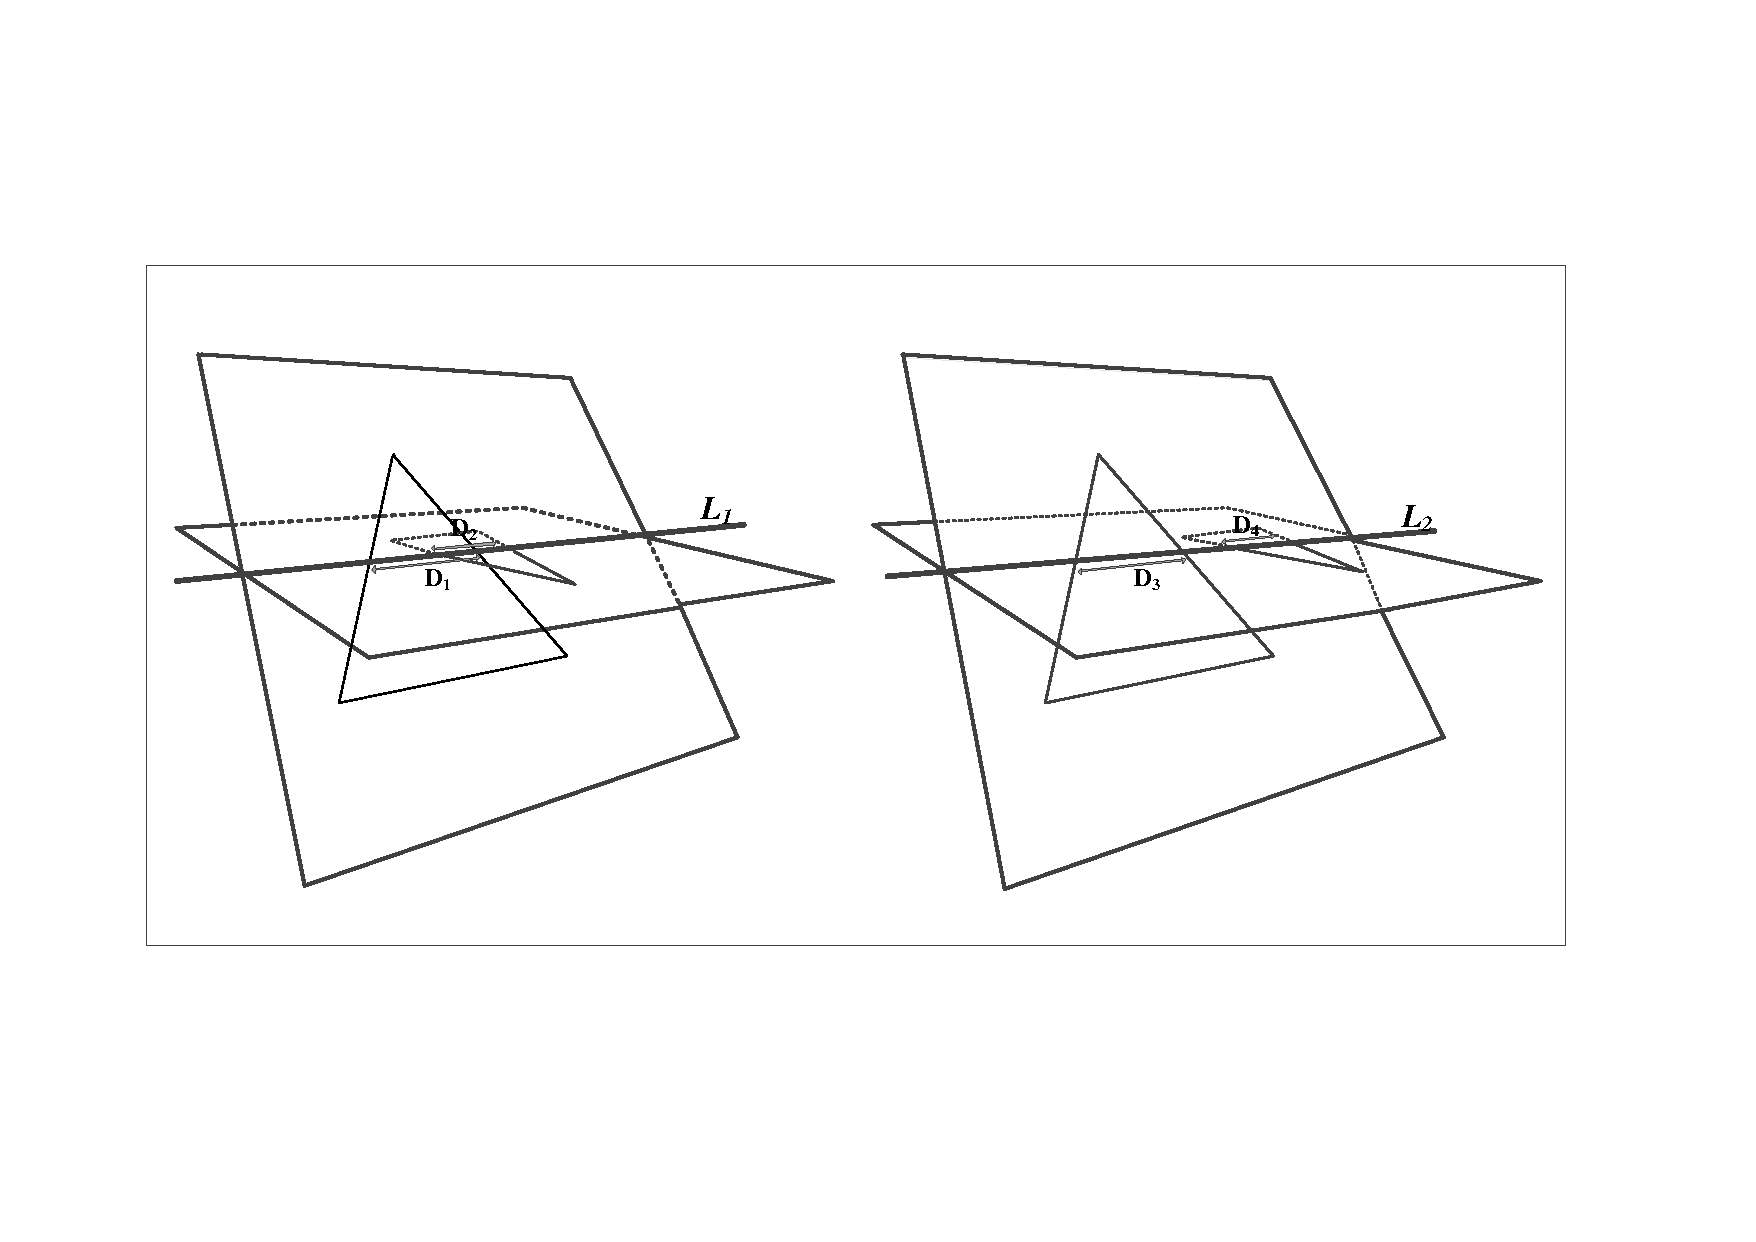
\includegraphics[width=5in]{TriangleTriangleTest.pdf}
    \caption{空间中两个非共面三角形的位置关系\cite{Moller1997}}
  \label{fig:two:triangle:ui}
\end{figure}

图~\ref{fig:two:triangle:ui}左图中,两个三角形所在平面交于直线~$\bm{L}_1$~且与三角形公共部分为线段~$\bm{D}_1$~,另一个三角形与~$\bm{L}_1$~交于线段$\bm{D}_2$,相应的右图两个三角形分别交公共交线~$\bm{L}_2$~于~$\bm{D}_3$~和~$\bm{D}_4$~,其中~$\bm{D}_1$~和~$\bm{D}_2$~相交可以推出两个三角形相交,反之~$\bm{D}_3$~和~$\bm{D}_4$~不相交因此三角形不相交,因此只需要判断两个三角形与平面交线的线段是否相交即可\cite{Moller1997},以下方法都基于此结论。

假设两个三角形~$T_1(\bm{U}_1,\bm{U}_2,\bm{U}_3), T_2(\bm{V}_1,\bm{V}_2,\bm{V}_3)$~所在平面分别为~$\Pi_1, \Pi_2$,
假设平面方程~
\begin{equation}
\Pi_1 = \bm{n}_1 \cdot \bm{x}+d_1 = (U_2 - U_1) \times (U_3-U_1)  \cdot \bm{x} + d_1,
\label{equa:tri:tri:plane}
\end{equation}
其中将任意一点~$U_i, i \in \{1,2,3\}$~带入公式~\ref{equa:tri:tri:plane}~得~$d_1$,同理得到~$\Pi_2$。

然后将~$T_2$~三个顶点带入方程~\ref{equa:tri:tri:plane}~得到~$T_2$~到~$\Pi_1$~的有向距离~$\bm{l}_{1i}, i \in \{1,2,3\}$,根据~$\bm{l}_{1i}$~的值共下面三种情况:
\begin{enumerate}[(1)]
  \item 若~$\forall i \in \{1,2,3\}, l_{1i} = 0$,即~$T_2$~的三个顶点到~$\Pi_1$~的距离都为0,则两个三角形共面;
  \item 若~$\forall i \in \{1,2,3\}, l_{1i} > 0$ 或~$\forall i \in \{1,2,3\}, l_{1i} < 0$,即有向距离同号,则~$T_2$~在~$\Pi_1$~的同侧,可立即排除相交;
  \item 其他情况,~$T_2$~必交~$\Pi_1$~于一条线段。
\end{enumerate}

同理可以根据~$T_1$~到~$\Pi_2$~得到类似的情况。针对情况(1),共面的两个三角形求交可以通过两个三角形中三条线段两两判定是否相交最多9次线段线段求交判定可得,或者通过我们在文献~\ref{linjianli2014}~中提出的方法进行,该方法对线段三角形的位置做了详细的分类可通过不超过~6~次线段线段求交判定;针对情况(2),计算出有向距离同号后即可排除相交立即返回;
针对情况(3),如图~\ref{fig:two:triangle:ui2}~所示,不妨设~$T_1$~中点~$\bm{V}_1, \bm{V}_2$~在平面~$\Pi_2$的一侧,$\bm{V}_3$~在另外一侧,
且点~$\bm{V}_1, \bm{V}_2$~在平面上投影点分别为~$\bm{K}_1,\bm{K}_2$,线段~$\bm{V}_1\bm{V}_2, \bm{V}_2\bm{V}_3$~与~$\bm{L}$~分别交于点~$\bm{I}_1,\bm{I}_2$,点~$\bm{V}_1,\bm{V}_2$~向直线~$\bm{L}$~的投影点分别为~$\bm{P}_1,\bm{P}_2$,
三角形~$T_1$~交于直线~$\bm{L}$~与线段~$\overline{I_1I_2}$。%,现在目的是求$I_1I_2$。

\begin{figure}[htbp]
  \centering
    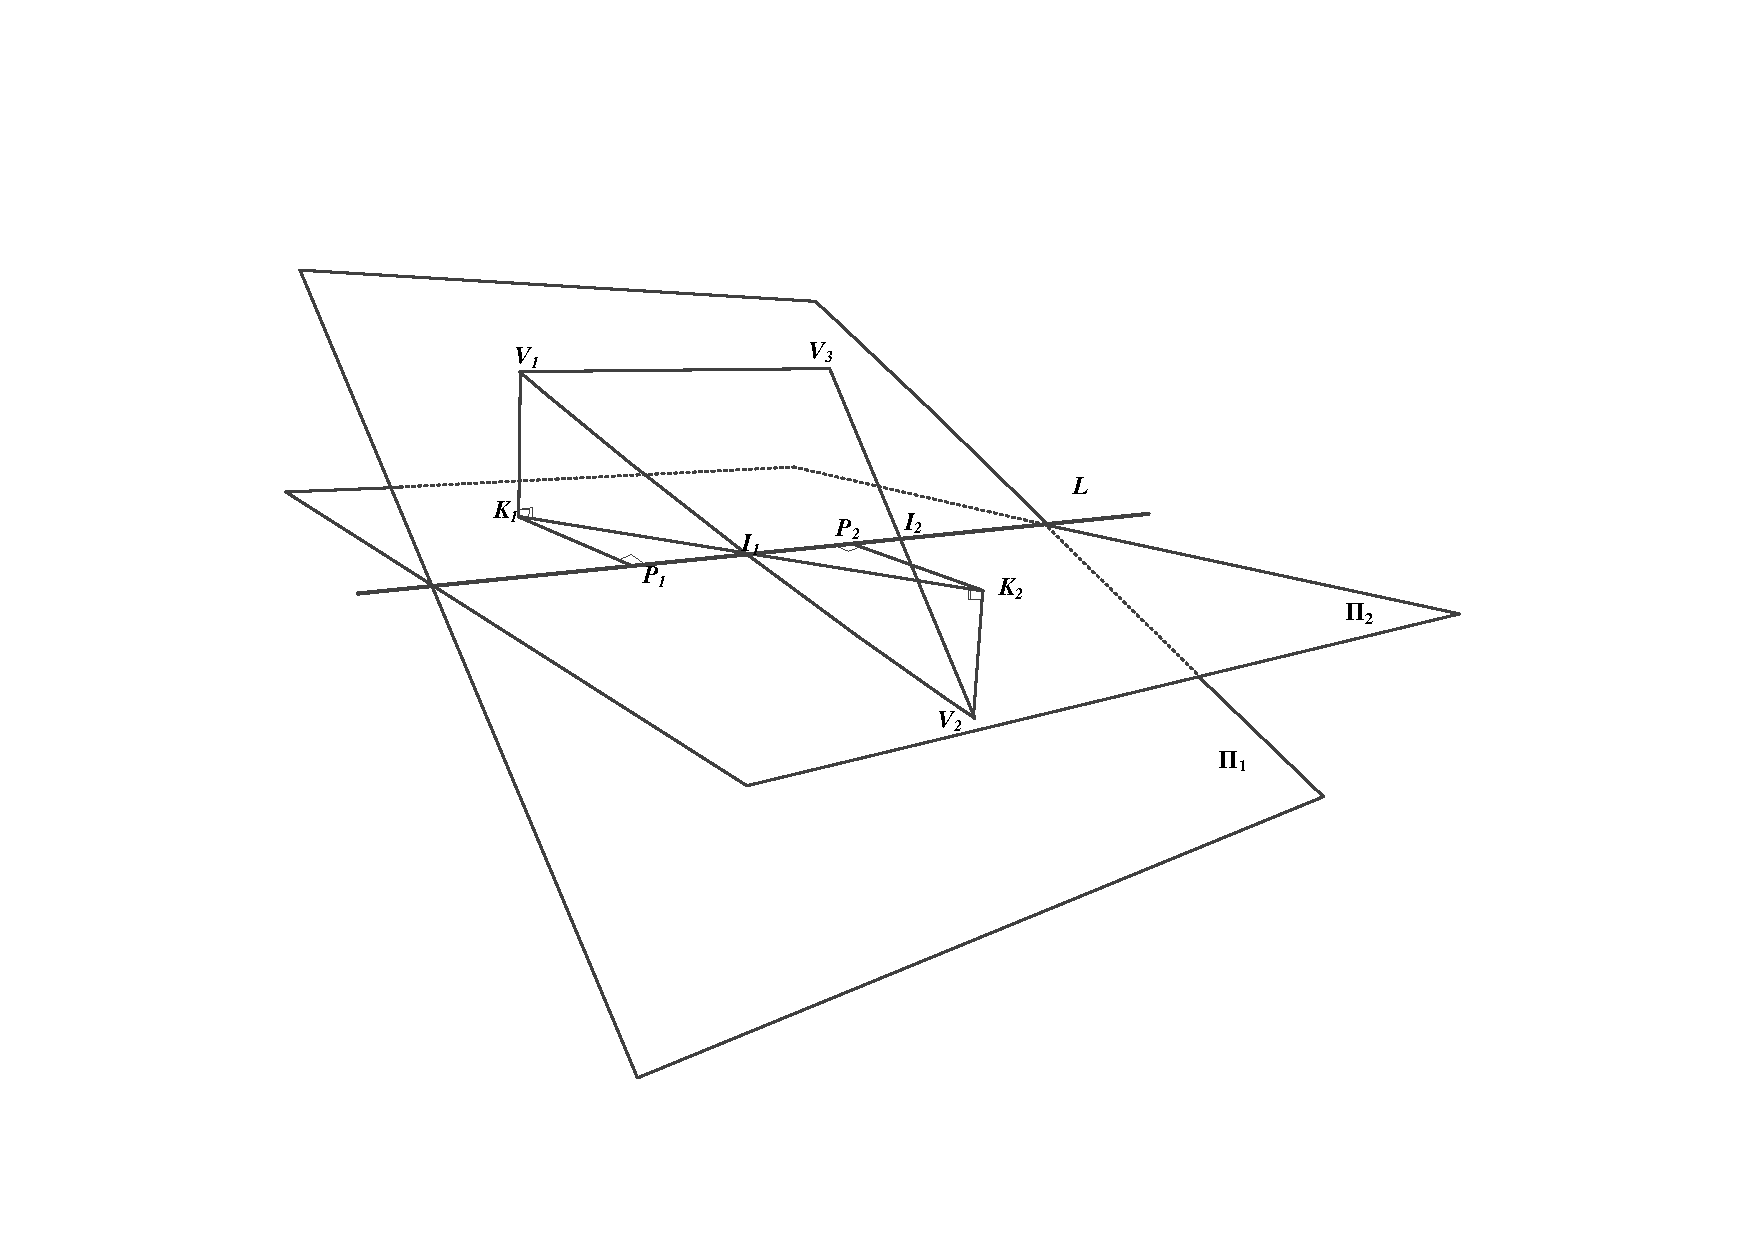
\includegraphics[width=4in]{TriangleTriangleTest2.pdf}
    \caption{求非共面三角形区间线段示意图\cite{Moller1997}}
  \label{fig:two:triangle:ui2}
\end{figure}

已知直线~$\bm{L}$~的方向为$\bm{n}_L = \bm{n}_1 \times \bm{n}_2$,设~$\bm{O}$~为~$\bm{L}$上一点,则直线的参数方程为
$\bm{L} = t \cdot \bm{n}_L + \bm{O}$,假设交点~$I_1 = t_1 \cdot \bm{n}_L + \bm{O}$,投影点满足
$p_1 = \bm{n}_L \cdot(\bm{V}_1 - \bm{O}), p_2 = \bm{n}_L \cdot (\bm{V}_2 - \bm{O})$,由图~\ref{fig:two:triangle:ui2}~可知,
$\bigtriangleup K_1P_1I_1 \sim \bigtriangleup K_2P_2I_1, \bigtriangleup V_1K_1I_1 \sim \bigtriangleup V_2K_2I_1$,可得

\begin{equation}
  \frac{t_1 - p_1}{p_2-p_1} = \frac{l_{11}}{l_{11}-l_{12}} \Rightarrow \newline
   t_1 = (p_2-p_1)\frac{l_{11}}{l_{11}-l_{12}} + p_1
  \label{equa:triangle:intersectionline:param}
\end{equation}

同理可得~$\bm{I}_2$~的参数~$t_2$,三角形~$T_2$~用相同的方法也能得到区间的参数,即可判断两个区间线段是否相交,进而可得该非共面的两个三角形是否相交。
完整的算法如~\ref{alg:triangles:intersection}~所示。

\begin{algorithm}[htbp]
\small
\caption{三角形求交算法}
\label{alg:triangles:intersection}
\begin{algorithmic}[1]
\Require
两个三角形的6个顶点 $T_1(\bm{U}_1, \bm{U}_2, \bm{U}_3), T_2(\bm{V}_1, \bm{V}_2, \bm{V}_3)$
\Ensure
是否相交

\Function{TriangleTriangleDetection}{$\bm{U}_1, \bm{U}_2, \bm{U}_3, \bm{V}_1, \bm{V}_2, \bm{V}_3$}
    \State {$\Pi_1 \gets \bm{n}_1 \cdot \bm{x}+d_1$} \Comment{按照公式~\ref{equa:tri:tri:plane}~计算$T_1$所在平面方程}
    \For {$i = 1 \to 3$}
        \State {$l_{1i} \gets \bm{n}_1 \cdot \bm{V}_i + d_1$} \Comment {计算$T_2$到$\Pi_1$的有向距离}
    \EndFor
    \If {$(l_{11} > 0 \textbf{~and~} l_{12} > 0 \textbf{~and~} l_{13} > 0) \textbf{or}
          (l_{11} < 0 \textbf{~and~} l_{12} < 0 \textbf{~and~} l_{13} < 0)$}
          \State \Return \textbf{False} \Comment{$T_2$在$\Pi_1$的同侧,排除}
    \EndIf
    \If {$l_{11} = 0 \textbf{~and~} l_{12} = 0 \textbf{~and~} l_{13} = 0$}
        \State \Return \Call{EdgeEdgeTest}{$\bm{U}_1, \bm{U}_2, \bm{U}_3, \bm{V}_1, \bm{V}_2, \bm{V}_3$}
        \State \Comment{$T_2$与$T_1$的共面,普通的边边相交测试}
    \EndIf
    \State {$\Pi_2 \gets \bm{n}_2 \cdot \bm{x}+d_2$} \Comment{按照公式~\ref{equa:tri:tri:plane}~计算$T_2$所在平面方程}
    \For {$i = 1 \to 3$}
        \State {$l_{2i} \gets \bm{n}_2 \cdot \bm{U}_i + d_2$} \Comment {计算$T_1$到$\Pi_2$的有向距离}
    \EndFor
    \If {$(l_{21} > 0 \textbf{~and~} l_{22} > 0 \textbf{~and~} l_{23} > 0) \textbf{or}
          (l_{21} < 0 \textbf{~and~} l_{22} < 0 \textbf{~and~} l_{23} < 0)$}
          \State \Return \textbf{False} \Comment{$T_1$在$\Pi_2$的同侧,排除}
    \EndIf
    \State {$t_1 \gets \Call{CalParam}{}, t_2 \gets \Call{CalParam}$}  
    \Comment {按照公式~\ref{equa:triangle:intersectionline:param}~计算线段$\bm{D}_1$的参数区间} 
    \State {$t_3 \gets \Call{CalParam}{}, t_4 \gets \Call{CalParam}$}  \Comment{类似的方法计算线段$\bm{D}_2$的参数区间} 
    \If {$\Call{Overlap}{t_1, t_2, t_3, t_4}$}
       \State \Return \textbf{True} \Comment{区间交叉,表明三角形相交返回\textbf{True}}
    \Else
       \State \Return \textbf{False}
    \EndIf
\EndFunction

\end{algorithmic}
\end{algorithm}

算法~\ref{alg:triangles:intersection}~第~10~行在进行边边测试子过程中,可通过点与有向线段的位置关系确定,如线段两个端点都在另外一个有向线段的一边说明两线段不相交,反之相交,不需要求解出实际的交点。
在实际实现过程中,往往需要引入容差以提高算法的稳定性。文献~\onlinecite{Moller1997}~介绍了更多的优化技巧。

\section{基于 $k$-CBP 的碰撞检测算法}
\label{sec:cd:baseon:kcbp}

凸包围多面体可应用于加速相关几何算法的整体效率, 图~\ref{lbl:bunny-box-kcbp-collsion-detection-example}
为利用~Bunny~模型进行碰撞检测的示例, 图中模型~1~与~2、2~与~3~的包围盒分别相交, 而其~$16$-CBP~仅~1~与~2~相交, 实际模型仅~1~与~2~相交.
用~$16$-CBP~可排除模型~2~与~3~之间的碰撞检测, 而仅用包围盒算法则无法排除, 显然检测模型~2~与~3~的~$16$-CBP~是否相交比直接通过检测模型~2~与~3~是否相交更省时间.
%在碰撞检测算法中, 在进行真实模型的相交检测前一般会用包围球、包围盒等包围体进行预先排除$^{[17]}$.

\subsection{静止场景中的碰撞检测算法}
\label{subsec:static:cd}

\begin{figure}[htbp] 
\centering
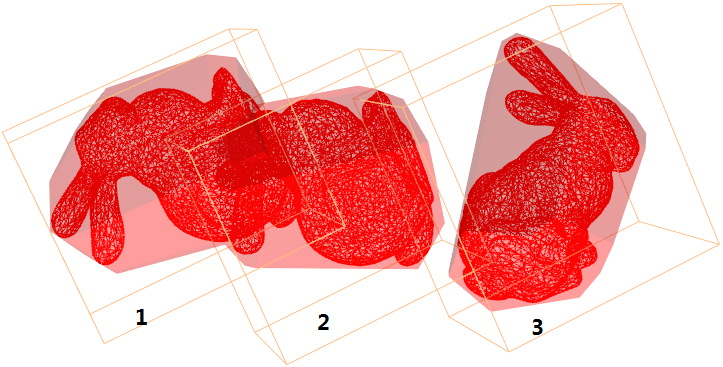
\includegraphics[width=5in]{bunny-box-kcbp-collsion-detection-example.png}
\caption{~$k-$CBP~应用于碰撞检测示例}
\label{lbl:bunny-box-kcbp-collsion-detection-example}
\end{figure}


模型的~$k$-CBP~相交后,会用模型的~AABB~树进一步对模型进行碰撞检测,模型的~AABB~树构造方法如第~\ref{subsec:kcbp:cd:aabb}~节所述,
图~\ref{fig:bunny:aabb:bvh:toplayer4}~是按照本文所采用的构造方法针对~Bunny~模型构造的~AABB~树形结构的顶上~4~层。

\begin{figure}[htpb]
  \centering
  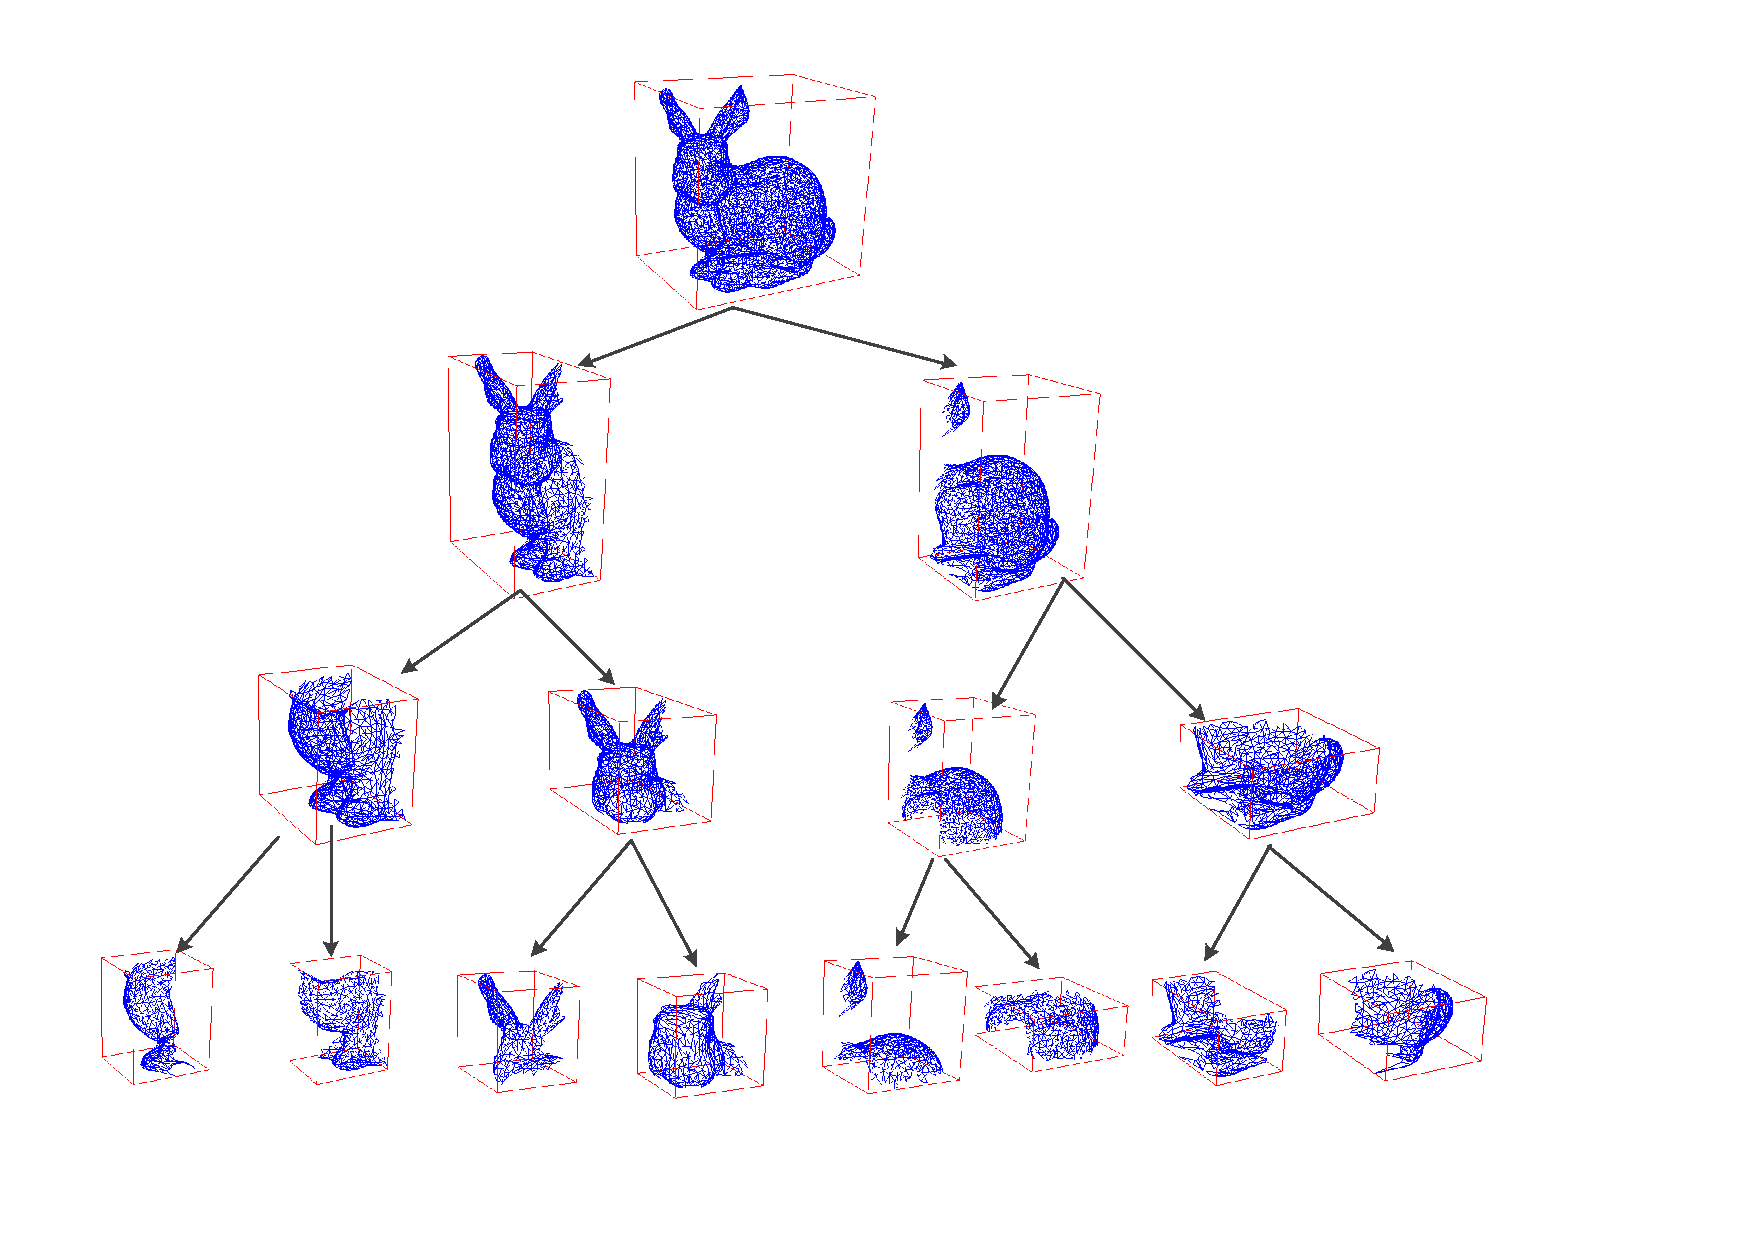
\includegraphics[width=\textwidth]{bunny-aabb-bvh-4-layers.pdf}
  \caption{Bunny~模型的~AABB~树形结构(部分)}
  \label{fig:bunny:aabb:bvh:toplayer4}
\end{figure}

整体的碰撞检测算法流程图如图~\ref{fig:flowchart:cd}所示,首先扫描所有输入模型点集,对每个模型计算其包围盒,然后计算要参与碰撞检测的模型的包围盒对进行相交测试,
假设要计算参与碰撞检测的模型的包围盒相交的对数为~$n_1$,再对这~$n_1$~对模型计算其~$k$-CBP~并进行初始化,如构造~AABB~树、初始化~GJK~算法,并计算~$k$-CBP
是否相交,此步骤后剩余模型对数为~$n_2$,最后再对这~$n_2$~对模型进行构造~AABB~树进而进行相交测试,真实模型相交对数为~$n_3$。整个流程中,包围盒的命中率为$n_1 / n_3$,$k$-CBP~的命中率为~$n_2/n_3$。


\begin{figure}[htpb]
  \centering
  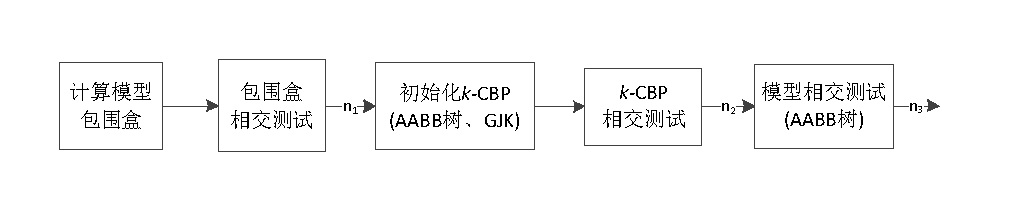
\includegraphics[width=\textwidth]{collision-detection-flowchart.pdf}
  \caption{碰撞检测算法流程图}
  \label{fig:flowchart:cd}
\end{figure}

\subsection{运动场景中的碰撞检测算法}
\label{subsec:moving:cd}

当在运动场景中的模型进行碰撞检测时,模型中的点坐标会更新,一种方法是重新计算模型中的所有点再对模型做碰撞检测,但当模型点数量较大时,此方法不可取;
另外一种算法是仍然利用静态场景中的~AABB~树形结构,仅重新计算将要碰撞的节点的坐标值,进而进行相交检测。
节点包围盒坐标在运动过程中发生变化,精确的包围盒是重新计算该节点包含原始模型的点在变化后的点坐标值的包围盒,本文利用一种近似算法即仅对包围盒的~8~个顶点进行转换
然后计算这8个顶点的包围盒,用这个近似包围盒进行遍历剪枝,当到叶子节点后,再重新计算网格模型的点的新坐标值用同样的方法进行相交检测。

模型围绕任意过原点的轴~$\bm{n}(x, y,
z)$~旋转任意角度~$\theta$~的变换矩阵如公式~\ref{equa:rotate:matrix}~所示,其中$\lambda
= 1-\cos\theta$,
详细的推导过程可以参考文献~\onlinecite{dunn20023d}。

\begin{equation}
%\small
\left\{
    \begin{array}{ll}
    \bm{R}(\bm{n},\theta) 
    &= 
          \cos\theta \begin{pmatrix}
                      1 & 0 & 0 \\
                      0 & 1 & 0 \\
                      0 & 0 & 1
                     \end{pmatrix}
          + \lambda \begin{pmatrix}
                    \bm{n}_x^2 & \bm{n}_x\bm{n}_y & \bm{n}_x\bm{n}_z \\
                    \bm{n}_x\bm{n}_y & \bm{n}_y^2 & \bm{n}_y\bm{n}_z \\
                    \bm{n}_x\bm{n}_z & \bm{n}_y\bm{n}_z & \bm{n}_z^2 
                    \end{pmatrix}
          + \sin\theta \begin{pmatrix}
                      0 & \bm{n}_z & -\bm{n}_y \\
                      -\bm{n}_z & 0 & \bm{n}_x \\
                      \bm{n}_y & -\bm{n}_x & 0
                      \end{pmatrix}
          \\
    ~&=  
        \begin{pmatrix}
            %\begin{array}{ccc}
              %\cos\theta+(1-\cos\theta)\cdot\bm{n}_x^2 & (1-\cos\theta)\cdot\bm{n}_x\cdot\bm{n}_y + \sin\theta\cdot\bm{n}_z & (1-\cos\theta)\cdot\bm{n}_x\cdot\bm{n}_z-\sin\theta\cdot\bm{n}_y \\
              %(1-\cos\theta)\cdot\bm{n}_x\cdot\bm{n}_y-\sin\theta\cdot\bm{n}_z & \cos\theta+(1-\cos\theta)\cdot\bm{n}_y^2 & (1-\cos\theta)\cdot\bm{n}_y\cdot\bm{n}_z+\sin\theta\cdot\bm{n}_x \\
              %(1-\cos\theta)\cdot\bm{n}_x\cdot\bm{n}_z + \sin\theta\cdot\bm{n}_y & (1-\cos\theta)\cdot\bm{n}_y\cdot\bm{n}_z - \sin\theta\cdot\bm{n}_x &  \cos\theta+(1-\cos\theta)\cdot\bm{n}_z^2 
              \cos\theta+\bm{n}_x^2\lambda & \bm{n}_x\bm{n}_y\lambda + \bm{n}_z\sin\theta & \bm{n}_x\bm{n}_z\lambda-\bm{n}_y\sin\theta \\
              \bm{n}_x\bm{n}_y\lambda - \bm{n}_z\sin\theta & \cos\theta+\lambda\bm{n}_y^2 & \bm{n}_y\bm{n}_z\lambda+\bm{n}_x\sin\theta \\
              \bm{n}_x\bm{n}_z\lambda + \bm{n}_y\sin\theta & \bm{n}_y\bm{n}_z\lambda - \bm{n}_x\sin\theta &  \cos\theta+\bm{n}_z^2\lambda 
          \end{pmatrix} \\
  \end{array}
\right.
\label{equa:rotate:matrix}
\end{equation}

当模型平移时,点~$\bm{P}(x, y, z)$~平移~$\bm{t}(t_x, t_y, t_z)$~后的点坐标为~$\bm{P}'(x+t_x, y+t_y, z+t_z)$,可用~$4 \times 4$~的变换矩阵~$\bm{T}$~表示,即
\begin{equation}
  \bm{T}(\bm{t}) =
  \begin{pmatrix}
    1 & 0 & 0 & t_x \\
    0 & 1 & 0 & t_y \\
    0 & 0 & 1 & t_z \\
    0 & 0 & 0 & 1 \\
  \end{pmatrix}
  \label{equa:translate:matrix}
\end{equation}

因此当模型平移旋转时产生的变换矩阵~$\bm{M}$~为
\begin{equation}
\bm{M}=\bm{R}(\bm{n}, \theta) \cdot \bm{T}(\bm{t}),
\label{equa:transform:matrix}
\end{equation}
AABB~节点包围盒更新后的算法如算法~\ref{alg:transform:box}~所示,
算法输入为平移向量$\bm{t}$及旋转方向和角度$\bm{n}, \theta$或者直接传入变化矩阵~$\bm{M}$~即可。

\begin{algorithm}[htbp]
\small
\caption{AABB节点包围盒更新算法}
\label{alg:transform:box}
\begin{algorithmic}[1]
\Require
AABB包围盒 $box$,
平移旋转变换矩阵$\bm{M}$
\Ensure
变换之后的包围盒 $box'$

\Function{TransformBox}{$box, \bm{M}$}
    \State $vertices \gets \Call{GetAABBVertices}{box}$ 
    \State $box' \gets \emptyset$
    \ForAll {$\bm{v} \in vertices$} \Comment{遍历~$box$~的8个顶点}
        \State {$\bm{v'}= \bm{M} \cdot \bm{v}$} \Comment{计算变换后的点坐标}
        \State $\Call{update}{box', \bm{v'}}$ \Comment{根据变换后的顶点~$\bm{v}$~更新$box'$}
    \EndFor
    \State \Return $box'$
\EndFunction
\end{algorithmic}
\end{algorithm}

运动场景中模型的碰撞检测算法如算法~\ref{alg:moving:cd}~所示,假设参与碰撞检测的两个模型中第一个运动且变换矩阵为~$\bm{M}$,第二个静止,
两个模型都运动时,可视第二个模型相对静止,将~$\bm{M}$~设置为第一个相对于第二个模型的相对变换矩阵。

\begin{algorithm}[htbp]
\small
\caption{运动场景中基于~AABB~树碰撞检测算法}
\label{alg:moving:cd}
\begin{algorithmic}[1]
\Require
两个模型~AABB~树的根节点 $root_0, root_1$ 及
平移旋转变换矩阵$\bm{M}$
\Ensure
模型是否相交 

\Function{MovingTraverseDetection}{$root_0, root_1, \bm{M}$}
    \State $mBox \gets \Call{TransformBox}{\bm{M}, root_0.box} $ \Comment{按照算法~\ref{alg:transform:box}~计算运动后的包围盒}
    \State $c \gets \Call{Intersect}{mBox, root_1.box} $
    \If {$c = \textbf{False}$}
        \State \Return \textbf{False} \Comment{包围盒不相交,直接返回\textbf{False}}
    \EndIf
    \If {$root_0.\Call{IsLeaf}$}
        \If {$root_1.\Call{IsLeaf}$} \Comment{两个叶子节点的原始几何进行相交测试} 
              \ForAll {$p_1 \in root_0.primitives$}
                  \ForAll {$p_2 \in root_1.primitives$}
                  \State \Return {$\Call{Intersect}{\bm{M}, p_1, p_2}$} \Comment{将$\bm{p}_1$应用于变换矩阵$\bm{M}$后采用算法\ref{sec:intersection:triangles}中进行三角网格相交测试}
                  \EndFor
              \EndFor 
        \Else
            \If {$\Call{MovingTraverseDetection}{root_0, root_1.left} \hspace{0.5em} \textbf{or} \newline \hspace{4em}
                \hspace*{5.5em} \Call{MovingTraverseDetection}{root_0, root_1.right}$} \hspace{2em}
                \State \Return \textbf{True}
            \EndIf
        \EndIf
    \Else
        \If {$root_1.\Call{IsLeaf}$}
            \If {$\Call{MovingTraverseDetection}{root_0.left, root_1} \hspace{0.5em} \textbf{or} \newline \hspace{4em}
                 \hspace*{5.5em} \Call{MovingTraverseDetection}{root_0.right, root_1}$}
            \State \Return \textbf{True}
            \EndIf
        \Else \Comment{两个节点都有孩子节点}
            \If {$\Call{MovingTraverseDetection}{root_0.left, root_1.left}  \hspace{0.5em} \textbf{or} \newline \hspace{4em}
                 \hspace*{5.5em} \Call{MovingTraverseDetection}{root_0.left, root_1.right} \hspace{0.5em} \textbf{or} \newline \hspace{4em}
                 \hspace*{5.5em} \Call{MovingTraverseDetection}{root_0.right, root_1.left} \hspace{0.5em} \textbf{or} \newline \hspace{4em}
                 \hspace*{5.5em} \Call{MovingTraverseDetection}{root_0.right, root_1.right}$}
                 \State \Return \textbf{True}
            \EndIf
      \EndIf
    \EndIf
    \State \Return \textbf{False}
\EndFunction
\end{algorithmic}
\end{algorithm}

算法~\ref{alg:moving:cd}~是一个递归算法,从~AABB~树的根节点起向底层进行深度优先遍历,当检测到运动后的模型的某两个叶子节点的包围盒相交时,遍历其三角网格的相交检测算法,在实际实现过程中,本文的叶子节点仅含一个三角网格。
运动模型的三角网格应用变换矩阵得到一个新的三角网格,同样用~\ref{sec:intersection:triangles}~的算法对新的三角网格进行相交测试。
除了用该递归算法外,也可对算法~\ref{alg:aabbtree:traverse:iterator}~进行稍许改动(只需改变包围盒检测和三角网格检测的函数)的迭代算法,此处不在赘述。

在基于~GJK~的~$k$-CBP~碰撞检测算法中,只需要改变算法~\ref{alg:gjk}~中~$Support$~子过程,将变换矩阵应用到原始顶点进行计算得到新的支持点即可,而在连续运动的模型碰撞检测过程中,
利用爬山法可以将支持点的搜索优化到常数时间复杂度\cite{bergen1999fast}。


\section{实验结果}
\label{sec:exper-cd}

\subsection{与包围盒过滤算法对比}
\label{subsec:exper:box:kcbp}

本文实验通过生成不同数量的模型(模型位置和旋转角度随机生成), 碰撞检测时首先判断包围盒是否相交, 然后判断凸包围多面体是否相交, 最后再判断实际模型是否相交.
凸包围多面体之间的碰撞检测时可采用文献~${[27]}$~中提到的方法,
本文案例中模型和凸包围多面体是否相交都采用了普通~AABB~树的方式进行判断,
从如表~\ref{tab:exp:box:kcbp:collsiondetection}~的实验结果可看出含有凸包多围体的模型之间的碰撞检测算法能显著提高整体应用的效率. 

%\begin{landscape} 横放,效果不好看, 还是将表头的单位去掉了
\begin{table}[htbp]
\caption{$k$-CBP~和包围盒应用于碰撞检测结果对比}
\label{tab:exp:box:kcbp:collsiondetection}
\centering
\begin{tabular}{lccccccl}
 \toprule[1.5pt]
  n& c(Box) & c($16$-CBP) &  t(Box) & t($16$-CBP) & r(Box) & r($k$-CBP) & n(Model) \\
  \midrule[1.0pt]
%  10 & 0.1 & 1.8 & 26.0  & 0.1 & 2 & 0 & 0\\
%  30 & 0.2 & 2.9 & 134.0  & 70.0 & 11 & 6 & 5\\
%  50 & 0.5 & 4.8 & 506.0  & 255.2 & 41 & 22 & 19 \\
%  70 & 0.4 & 4.8 & 901.1  & 492.5 & 77 & 42 & 34 \\
%  90 & 0.7 & 5.7 & 1324.0  & 734.7 & 110 & 63 & 46 \\
%  100 & 0.7 & 7.8 & 1481.0  & 870.7 & 127 & 73 & 55 \\
%  150 & 1.0 & 9.8 & 4153.1  & 2473.0 & 349 & 212 & 150 \\
%  200 & 1.6 & 12.8 & 8049.3 & 4430.9 & 685 & 394 & 281 \\
   10 & 0.1 & 1.8 &    26.0  & 0.1    & 0.00  & 100.00 & 0\\
   30 & 0.2 & 2.9 &   134.0  & 70.0   & 45.45 & 83.33 & 5\\
   50 & 0.5 & 4.8 &   506.0  & 255.2  & 46.34 & 86.36 & 19 \\
   70 & 0.4 & 4.8 &   901.1  & 492.5  & 44.16 & 80.95 & 34 \\
   90 & 0.7 & 5.7 &  1324.0  & 734.7  & 41.82 & 73.02 & 46 \\
  100 & 0.7 & 7.8 &  1481.0  & 870.7  & 43.31 & 75.34 & 55 \\
  150 & 1.0 & 9.8 &  4153.1  & 2473.0 & 42.98 & 70.75 & 150 \\
  200 & 1.6 & 12.8 & 8049.3  & 4430.9 & 41.02 & 71.32 & 281 \\
  \bottomrule[1.5pt]
 \end{tabular}
\end{table}
%\end{landscape}

如表~\ref{tab:exp:box:kcbp:collsiondetection}~所示,
其中~n~表示场景中模型的数量, c(Box), c($16$-CBP)分别表示模型包围盒的构造时间和凸包围16面体的构造时间(单位ms)\footnote{此处的时间为得到一个$k$-CBP后直接通过应用变换矩阵得到新的$k$-CBP总时间且是利用~GPU~搜索截面的时间,后文与~$k$-DOP对比均采用~CPU~算法实现}, t(Box), t($16$-CBP)~分表表示用包围盒进行碰撞检测和利用凸包围16面体进行碰撞检测所耗费的时间,
其中~r(Box), r($16$-CBP)分别表示包围盒、16-CBP~的命中率(即用实际模型相交的数量除以包围体检测出来相交的数量), ~n(Model)模型实际相交的数量, 显然计算模型包围盒所耗费的时间要明显少于计算凸包围多面体的时间, 但由于凸包围多面体比包围盒紧致,
因而命中率比包围盒高, 能排除更多本不相交的模型进而节省碰撞检测总时间, 提高算法效率。该部分工作已经发表,详细内容见参考文献~\onlinecite{tanglei2014}。

\subsection{静止场景中与~$k$-DOP~算法对比}
\label{subsec:exper:kdop:kcbp:static}

为了和K-DOP进行对比,相同模型,kcbp也与kdop一样扫描点击重新构造,且都是用CPU实现的算法。


\subsection{运动场景中与~$k$-DOP~算法对比}
\label{subsec:exper:kdop:kcbp:dynamic}

为了和K-DOP进行对比,相同模型,kcbp也与kdop一样扫描点击重新构造,且都是用CPU实现的算法。
